\chapter{Results \& Discussion}\label{sec:results}

\section{Communication Results}

\subsection{Message Transmission}

Running tests to quantify the quality of communications between Cublis and Computer, we obtain the data in Figure \ref{img:comStats}. Specifically, these numbers where obtained through testing of the sync protocol.

\begin{figure}[H]
   \centering
   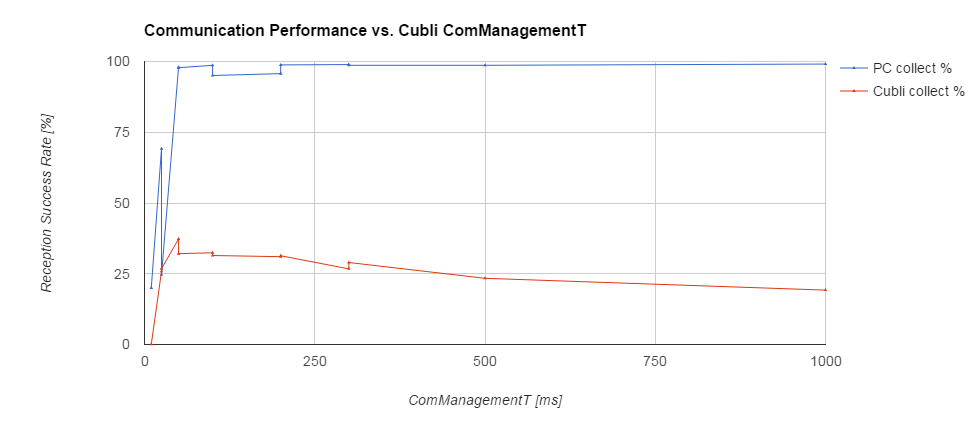
\includegraphics[width=1\textwidth]{img/comStats.png}
   \caption{A measure of the average communications success rate, with varying communication-update periods in Cubli.}
   \label{img:comStats}
\end{figure}

As such we observe that on average, there is a 30\% chance of Cubli collecting a message. This further means that if we are to send Cubli the same message 5 times, the probability of at least one message being successfully received is 85\% and for 10 identical messages, the same probability becomes 97\% .\\

In addition, tests were ran at 50 ms ComManagementT Delay, replacing the wireless adapter with a direct wired connection to the PC, and over a large amount of messages the resulting success rate for reception in Cubli increased to 50\%. It is therefore hypothesized that the remaining 50\% of losses originate from inside the software, particularly the way that UART reception is handled.\\

Running similar test during other protocols yields similar results, with Cubli's reception rate rarely exceeding 40\%.\\

A rare but several times observed occurrence was a crash of the Cubli software, the cause of which was not identified when debugging. Likelihood of this event increase with the communications volume and frequency, although it remains generally low and hard to predict.\\

Finally, through all the tests , and the whole project, messages from two Cublis were never observed to have mixed with one another. As the probability of such an occurrence was expected to be low, this is not such a surprise. However it shows that the order of magnitude of that likelihood is even smaller than expected - certainly due to the short time of UART emission at the Baud rate of 115200 bits per second. \textit{ Thought experiment: At a 100 bits per message, in theory such a baud rate implies that it takes 0.8 ms to send a message. Knowing that Cubli sends a message at most once every 50 ms with the current settings, the chance of two Cublis accidentally sending a message at the same time can be (very) approximately calculated as $\frac{0.8}{50}$, that is 1.6\% }.

\textbf{Addendum:} the code responsible for low reception rates in Cublis having been found, new communications performance for the Cubli are similar to that of the computer (that is, around 90\%). Since the low reception rates were relevant during the development phase, they remain mentioned in this report.

\subsection{Protocol Effectiveness}

Knowing the rate at which single messages are statistically dropped, it is interesting to quantify the success of communication protocols in ensuring complete and timely transfer of data between devices. \\

\textbf{The connecting protocol} was tested by pressing the '+' button, with two powered-on Cublis. Out of 100 attempts, 86 completed successfully, that is with all cubes marked as connected. A second trial was made, wherein 88 out of 100 attempts completed successfully.

With only one Cubli powered-on, the same test yielded a result of 99 out of 100 attempts successful.\\

Thus on average, the statistical success rate of the protocol with one Cubli is approximately 99\%, whereas with two Cublis it drops to 87\%. \\

This drop in performance was expected, and the likely cause is shadowing of a Cubli's messages by another. As explained previously, when two messages reach the application in quick succession, only the first one is treated - in order to stop the application from lagging behind - which leads to the observed behavior. \\

Adding more Cublis would arguably further degrade the performance, at which point it should become reasonable to implement time-slots during which only one Cubli is allowed to communicate. \textit{ For future endeavors, } this would be an interesting avenue of experimentation - however, it would require an accurate timekeeping mechanism, which is not yet available in the Cubli software. Another possibility which was considered, is to have the application only prompt one Cubli at a time, and whenever possible have Cublis only speak when prompted. This solution is however less general ( for example it does not apply for scenarios where Cublis must notify the application of failures, or similar cases. ), and would not be appropriate as a standard solution if future projects delve into making Cublis interact with each other independently from a computer, and symmetrically. Note however that the sync protocol developed in this project, for example, follows that principle ( only one Cubli talking at once ). \\

\textbf{The sync protocol}, when tested, completed successfully ( i.e. before the timeout delay ) 100 times, out of a 100 attempts. Failure has anecdotally been observed to occur in the event of a Cubli crash, which could not be repeated during the tests.\\

Because timeline syncing is sequential, that is, only one Cubli is synced at a time, the success rate is not heavily affected by the presence of multiple cubes - outside of the probabilistic combination of several events, i.e. the probability of two Cublis syncing correctly is a square of the probability for one Cubli.\\

\textbf{The choreography initating sequence}, when tested, has completed successfully 20 times out of 20. Testing was conducted using two cubes. Through non-experimental use, failures of the protocol are sometimes, though rarely observed. Thus, the success rate of this protocol can conservatively be considered to lie between 90\% and 100\%. \\

\textbf{The choreography failure sequence} could not be rigorously tested. Due to the complex and time sensitive nature of the communications it contains, it is expected that its failure rate is similar to the choreography initiating sequence with only one cube, and increases as more cubes are involved. This concurs with what is regularly observed in practice.

\section{Concept Validation}

At this point, the choreographer app is functional; Choreographies can be created and performed by Cublis - demonstrated with more or less reliability, depending on the amount of Cublis and the communications success rate.\\

As such, it can be reasonably concluded that the concepts which this project set out to develop are valid and practical.    

\begin{figure}[H]
   \centering
   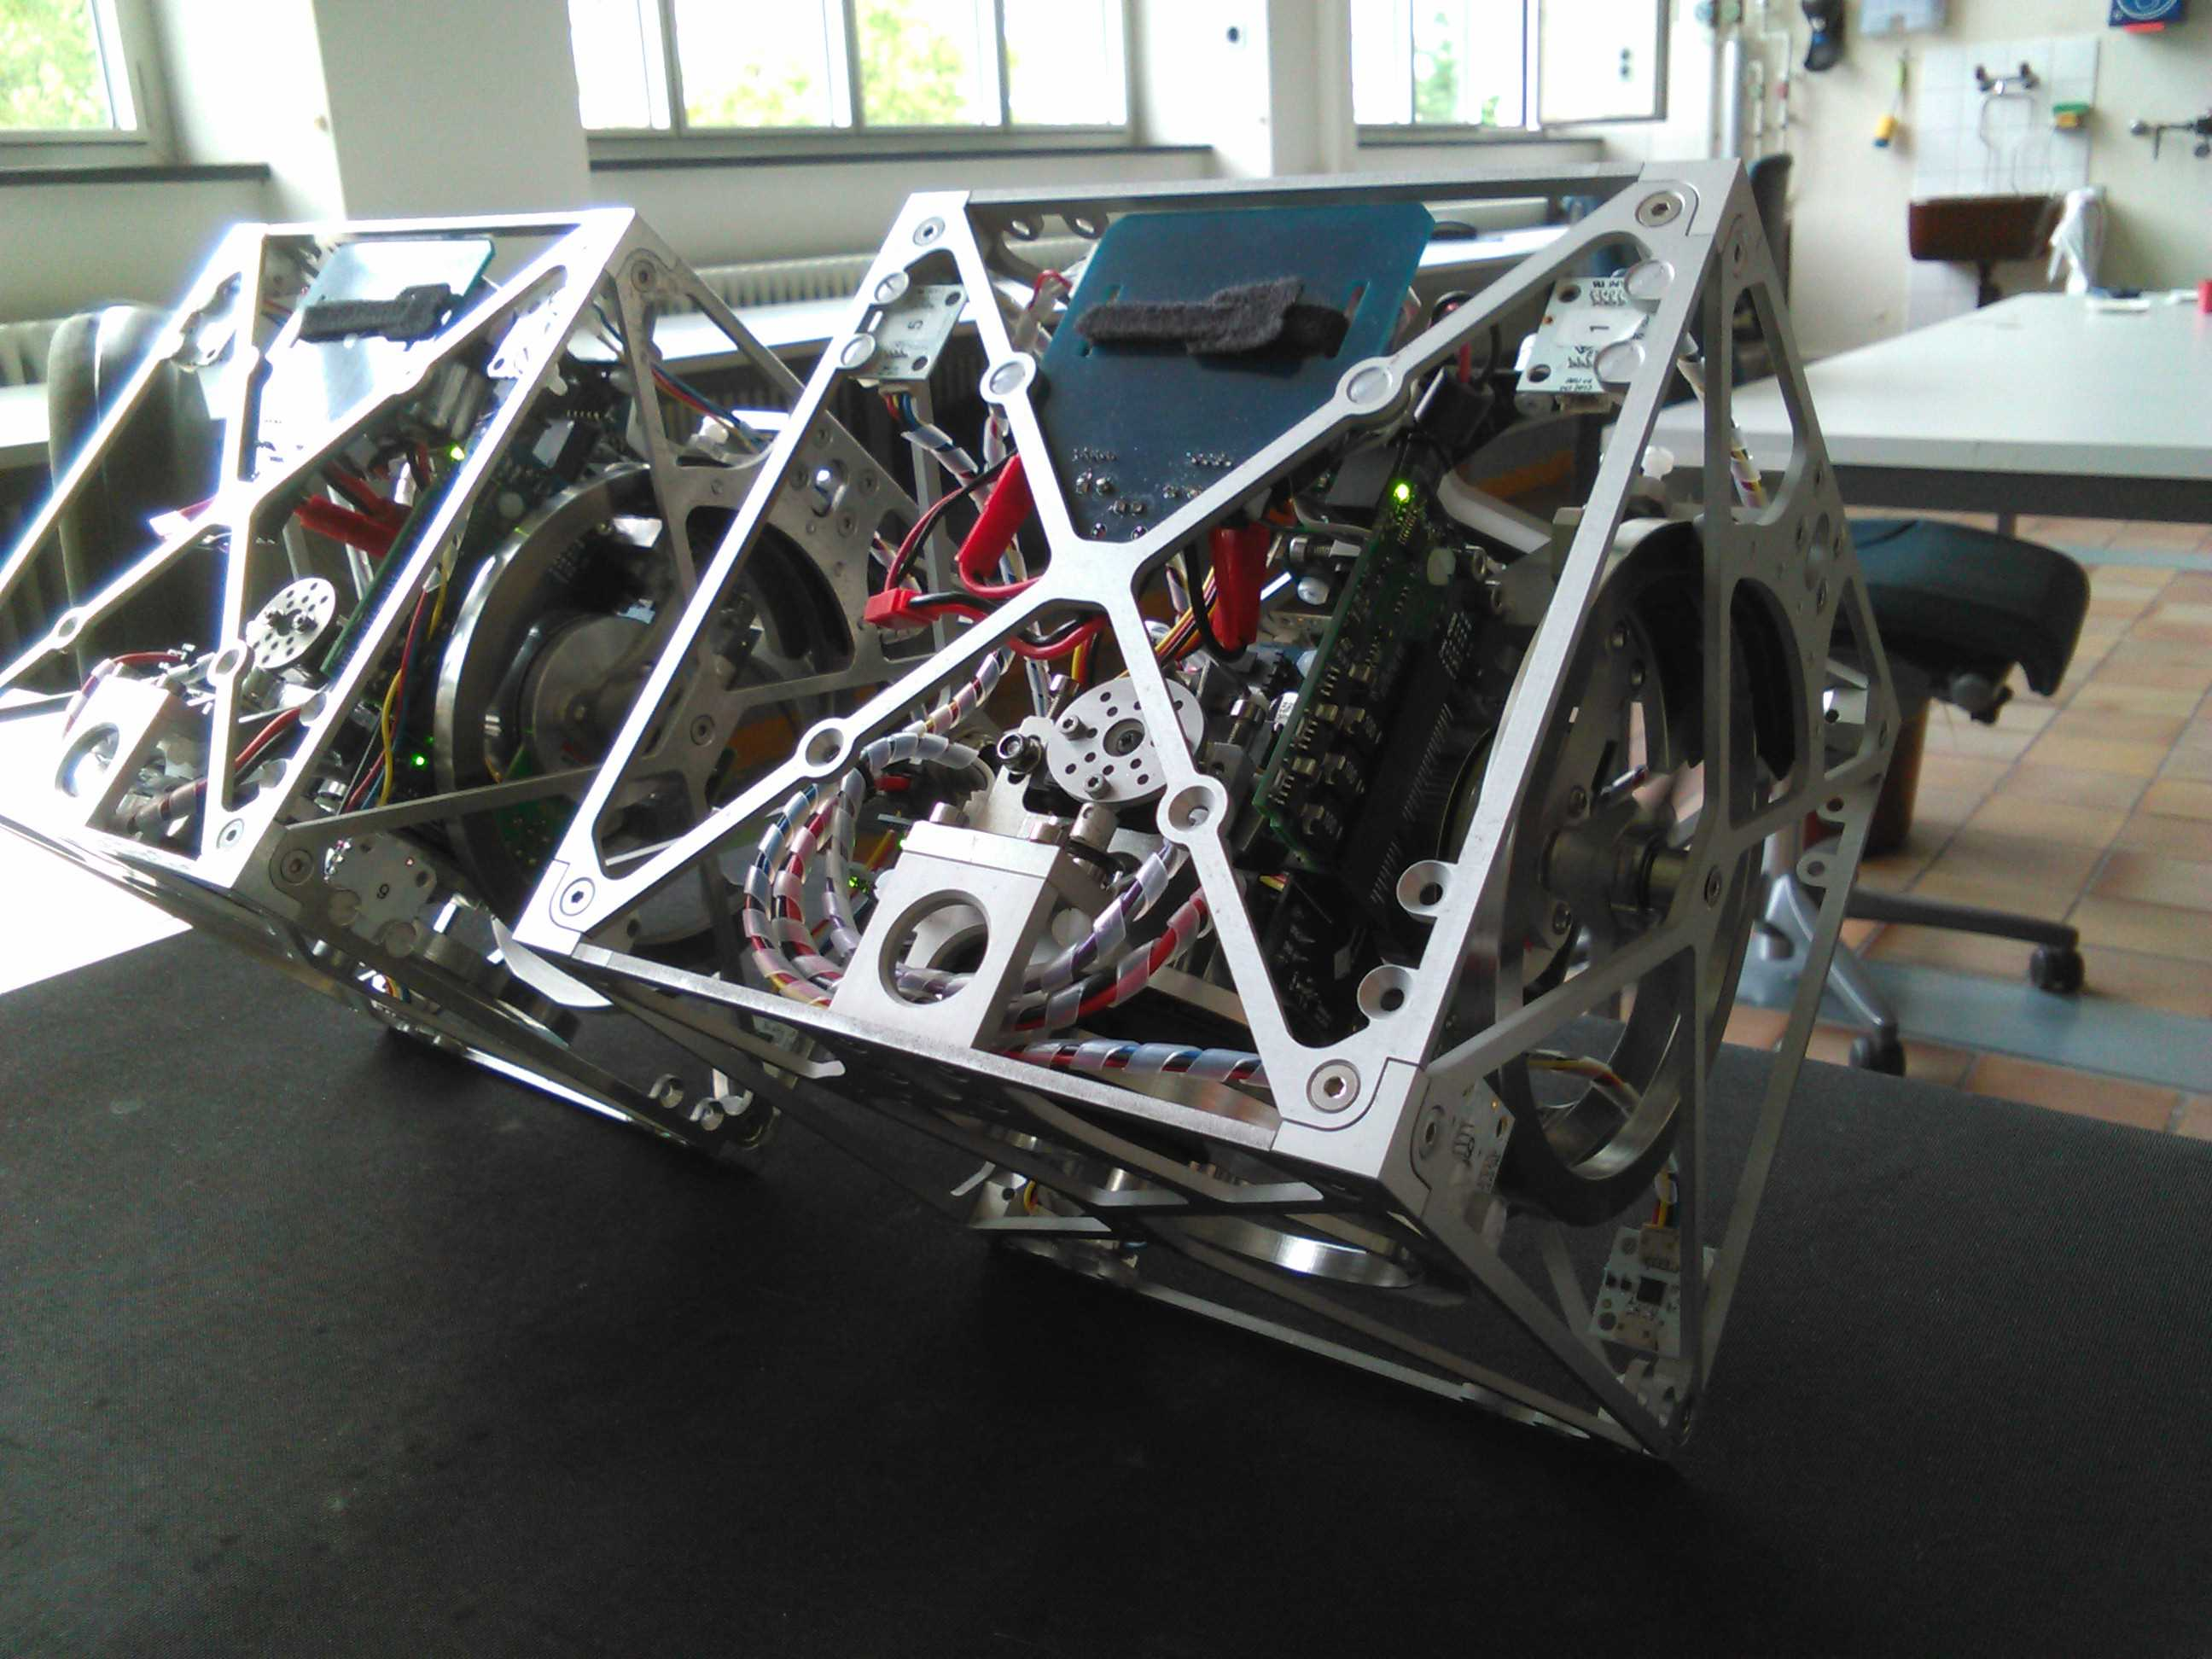
\includegraphics[width=1\textwidth]{img/Performing.jpg}
   \caption{Two Cublis jumping in sync during a choreography in the IDSC lab.}
   \label{img:performing}
\end{figure}

Much has been learnt in the process, and it is hoped that the efforts to augment Cubli continue after the completion of this project.

\section{What's next}

This project having reached its end, the outlook towards future Cubli possibilities is optimistic. Each conceptual goal developed, and fulfilled, has created potential avenues of innovation, and inspired ideas for future work on making Cubli an ever more capable robot.\\

A few examples which could be considered promising are detailed here:

\begin{itemize}
\item Jumping from any face/slanted position. Though this would require a more general approach in the controller tasks, it would allow Cubli to be independent from human intervention in almost all movement scenarios. It is estimated that the main necessary steps to undertake in order to implement this capability are : - outlining current face, edge, or corner based on IMU measurements. - use an angle system-state which is normalized to the current face.

\item Very little computer intervention - interactive Cublis. The main obstacle to overcome in order to achieve this capability is the communications failure rate. Barring that, emphasis can  be made on communications between Cublis rather than between Cubli and computer. The code developed during this project has generally been designed to enable the future implementation of these abilities.

\item Defining not just actions but movements ( go from A to B, head towards Cubli 1, ... ). Also an augmentation of Cubli intelligence, the algorithms necessary to adapt cube movements and resulting changes of coordinate systems into broader actions would certainly be interesting to develop. Resulting behavior could open up the door to new possibilities especially  if combined with the other examples presented here.

\end{itemize}

\section{Acknowledgements}

Thanks go to the IDSC team, for all the help in the face of difficulties, bugs, computer whims, and challenges.



